\documentclass[a4paper]{usiinfbachelorproject}

\captionsetup{labelfont={bf}}
%%%%%%%%%%%%%%%%%%%%%%%%%%%% PACKAGES %%%%%%%%%%%%%%%%%%%%%%%%%%%%%
\usepackage{todonotes}
\usepackage{float}

\usepackage[cache=false]{minted}

\usepackage[T1]{fontenc}
%\usepackage{moreverb}

%%%%%%%%%%%%%%%%%%%%%%%%%%%%%%%%%%%%%%%%%%%%%%%%%%%%%%%%%%%%%%%%%%%


%%%%%%%%%%%%%%%%%%%%%%%%% CUSTOM COMMANDS %%%%%%%%%%%%%%%%%%%%%%%%%
\newcommand{\projectName}{\_\_PROJECT\_\_NAME\_\_}

\usemintedstyle{xcode}


\newmintedfile[tsfile]{ts}{
linenos,
tabsize=4,
frame=lines,
breaklines=true,
xleftmargin=20pt
}

\newminted[tscode]{ts}{
linenos,
frame=lines,
tabsize=4,
breaklines=true,
xleftmargin=20pt
}

\newmintinline[ts]{ts}{
linenos,
frame=lines,
breaklines=true,
xleftmargin=20pt
}

%%%%%%%%% HTML

\newmintedfile[htmlfile]{html}{
linenos,
tabsize=4,
frame=lines,
breaklines=true,
xleftmargin=20pt
}

\newminted[htmlcode]{html}{
linenos,
frame=lines,
tabsize=4,
breaklines=true,
xleftmargin=20pt
}

\newmintinline[html]{html}{
linenos,
frame=lines,
breaklines=true,
xleftmargin=20pt
}

%%%%%%%%% JSON

\newmintedfile[jsonfile]{json}{
linenos,
tabsize=4,
frame=lines,
breaklines=true,
xleftmargin=20pt
}

\newminted[jsoncode]{json}{
linenos,
frame=lines,
tabsize=4,
breaklines=true,
xleftmargin=20pt
}

\newmintinline[json]{json}{
linenos,
frame=lines,
breaklines=true,
xleftmargin=20pt
}

\newmintedfile[scalafile]{scala}{
linenos,
tabsize=4,
frame=lines,
breaklines=true,
xleftmargin=20pt
}

\newminted[scalacode]{scala}{
linenos,
frame=lines,
tabsize=4,
breaklines=true,
xleftmargin=20pt
}

\newmintinline[scala]{scala}{
linenos,
frame=lines,
breaklines=true,
xleftmargin=20pt
}

%%%%%%%%%%%%%%%%%%%%%%%%%%%%%%%%%%%%%%%%%%%%%%%%%%%%%%%%%%%%%%%%%%%





\author{Your Name}

\title{\projectName}
\subtitle{The (optional) subtitle}
\versiondate{\today}

\begin{committee}
%With more than 1 advisor an error is raised...: only 1 advisor is allowed!
\advisor[Universit\`a della Svizzera Italiana, Switzerland]{Prof.}{Michele}{Lanza}
%You can comment out  these lines if you don't have any assistant
\assistant[Universit\`a della Svizzera Italiana, Switzerland]{Dr.}{Luca}{Ponzanelli}
\assistant[Universit\`a della Svizzera Italiana, Switzerland]{Dr.}{Andrea}{Mocci}
\end{committee}

\abstract {
An abstract describing what the prospectus is all about. ``Omit needless words'' \cite{Stru1899a}: It should fit within the page without making the footer of the title page break the page --- otherwise what kind of abstract would it be?
}




\begin{document}
%\maketitle

% Chapters
%%%%%%%%%%%%%%%%%%%%%%%%%%
\section{Introduction} \label{introduction}
%%%%%%%%%%%%%%%%%%%%%%%%%

\subsection{General issues}

Latex is not so complex. If you aren't familiar with it just spend some time in googling for latex commands (e.g. font formats, tables, figures, items,\dots).

\subsection{Getting started}
In order to use the bachelor thesis template, be sure that the following files are present in your working directory:
\begin{itemize}
\item usiinfbachelorproject.cls (The latex template)
\item logo-info.pdf (The logo figure)
\item references.bib (The references file)\\
\end{itemize}

\subsection {Compilation issues}

If you are not familiar with Tex, I advise you to download TexShop for Mac OS.\\
To include the references and display them in the final pdf, you have first to typeset this file with \textit{LaTex} (ComboBox upper left, if you use TexShop), then with \textit{BibTex} and finally again with \textit{LaTex}.\\
In order to resolve figures/table/\dots~references you have to run 2 times the (latex) typeset.

\subsection {Document structure}

Some basic sections:
\begin{itemize}
\item Introduction (including Motivation)
\item State of the Art
\item Project requirements and analysis
\item Project design (top-down)
\item Implementation issues (bottom-up)
\item Tests (methodology, results, comments)
\item Conclusions and future work or possible developments
\end{itemize} 

\subsection {Some examples}

\textbf{Figure ~\ref{fig:USILogo}} shows how to insert figures in the document.

\begin{figure} [h]
\centering

\includegraphics[width=0.5\textwidth]{Other/logo-info.pdf}
\caption{Caption of the figure}
\label{fig:USILogo}
\end{figure}

\noindent\textbf{Table \ref{tab:numbers}} shows how to insert tables in the document.

\begin{table}[h]
\centering
\scalebox {0.8} {
\begin{normalsize}\begin{tabular}{l|lll}
\textbf{Col 1} & \textbf{Col 2} & \textbf{Col 3} & \textbf{Col 4}\\
\hline
1 & 2 & 3 & Goofy\\
4 & 5 & 6 & Mickey
\end{tabular}
\end{normalsize}
}
\caption{Caption of the table}
\label{tab:numbers}
\end{table}




\section{Introduction}\label{sec:introduction}
From the advent of new languages, frameworks and methodologies, the way software is started, developed and maintained has dramatically shifted from what it was. Therefore, developers need to be able to keep up with the evolution, which requires consulting the documentation, understanding new principles, and in the end being able to be productive. 

This process is not only straining, it is also time consuming. This is due to the fact that the developer has to consult the documentation to understand new concepts as well as watch out for breaking changes that may be introduced at a moments notice. 

Luckily in the current age there are multiple ways to obtain information. From simple web searches, all the way to forums and Q\&A websites such as Stack Overflow, the developer in question is able to quickly understand stay update on new technologies, languages, etc. %what steps have to be taken in order to correct possible bugs, or to altogether prepare for major version changes. 

This availability of information can be a double edged sword. Where in the majority of cases a developer may be able to solve issues quickly because someone may already have encountered, there may be situations where the solution may be buried inside documents that do not directly treat the topic at hand. This causes the developer to be overloaded with information that is not pertinent to the task at hand, causing her to be less productive.

The goal of this project is to develop a tool that is able to summarise the contents of a page, and integrating it into the LIBRA\cite{Ponz2017a} recommender. This will allow the developer to choose the amount of information she may like to see, going from the entire contents, all the way to seeing only one paragraph of the document. The strategy consists in taking an algorithm such as LexRank, augmenting it in order to support the heterogeneous nature of development artefacts, which may not only include text, but also code.



\section{State of the art}\label{sec:stateOfTheArt}
\todo[inline]{Still a major TODO...}
\newpage
%\subsection{Recommender Systems}
%The idea of a recommender ties directly into one of a summariser. The correlation is easy to see: both approaches try to show the end user relevant information that has to do with the current context. We start by analysing some currently existing recommender systems.
%
%Recommender systems have existed for quite a while, outside of Software Engineering. Firms like Ebay, Amazon and many other online stores have been showing clients related and potentially interesting purchases. The data is usually computed using the previous purchases, related searches, and data from other clients that have looked at the same item. 
%
%Another example is streaming services, such as Netflix or Spotify. Both of these services show the user what they may like, based on the history of a particular user, trending content, newly released material, etc. 
%
%These suggestions are tailored to the user and tend to be accurate. We can deduce that these systems may be holistic in their implementation, being as they do not only consider the current item, but many other factors such as user history
%
%Looking at Software engineering, the principle is still the same: recommend to the developer relevant documentation, questions, examples that may help in solving the current problem. However, what these systems also bring is information overload. By showing the developer more and more information, she may be overwhelmed by the sheer amount of it, causing more confusion. This is where summarisation plays a key component.
%
%\subsection{Summarisation}

\section{Project requirements and Analysis}\label{sec:requirementsAndAnalysis}


\subsection{Challenges}
As previously stated, the goal of this project is to reduce the overload of information experienced by a developer when searching for information online. While this is a challenge in itself, there are multiple other non-trivial challenges:

\begin{itemize}
\item {\bf Lack of structure}\label{sec:lackOfStructure}\\
In general, each website is implemented in a different structure. Although the HTML constructs are the same, there are no strict rules in how they should be used. %To overcome this challenge, ad-hoc parser were created for each website, aiding in understanding how to extract the relevant information, to then be sent the the service, as discussed in section \ref{sec:architecture}.
\item {\bf Integrity of information}\\
Users will mostly have to deal with documents that may contain code snippets. Many websites tend to include code, which helps in the explanation of the problem at hand. Due to this heterogeneous nature of the information, these section had to be kept intact.

\end{itemize}

\subsection{HoliRank}

HoliRank \cite{Ponz2017a} is an algorithm that builds on top of LexRank \cite{Erkan:2004:LGL:1622487.1622501}, which itself is based on PageRank \cite{ilprints422}. 
Before we go any further, we describe how both LexRank and PageRank work from a high level perspective. PageRank simulates a random surfer, a user which randomly surfs the web clicking on links and never going back until it gets bored and starts from another random page. This random surfer is defined by the following formula:

\begin{equation}
PR(p_i) = \frac{1-d}{N}+ d\sum\limits_{p_j\in M(p_i)}\frac{PR(p_j)}{L(p_j)}
\end{equation}
where $d$ is a damping factor (usually set to 0.85), $M(p_i)$ is the set of all pages that link to $p_i$, $L(p_j)$ is the number of outgoing links from $p_i$, and $N$ is the total number of pages in the network and serves as a normalisation factor. In this approach, the probability that the random surfer may visit a page represents the degree of centrality of this page in a network of pages.

In order to move to LexRank, some modifications are needed. Instead of considering a network of pages, the approach considers a document as a collection of sentences that form a network. Then, PageRank is applied to this network of sentences. This modification to the algorithm allows for sentences, which in theory have no proper link between them, to be connected and used. 

In theory, LexRank could have been used ``as is'' to perform summarization, as most of the documents developers will consult are mainly composed of text. Issues arise when the page being viewed contains artifacts which are not purely text-based, such as code snippets. The difference between the data can cause issues when LexRank determines the similarity between the artifacts, since it does so by considering the pure textual similarity of the artifacts, which hinders the whole information provided by source code. The approach followed by HoliRank is to consider the heterogeneous nature of information in software engineering, i.e. the possibility of an artifact to be composed of either text or code. By performing this distinction, the algorithm is able to access the multiple layers of information provided by the different artifacts, since the way similarity is calculated varies depending on the type of the artifact. 
\section{\projectName}\label{sec:projectDesign}
\subsection{Overview}
As described in section~\ref{sec:introduction}, the goal of this project is to reduce the amount of information presented to the developer, to reduce the overload that is introduced by the amount of information that is readily available.

In order to do so, we have developed \projectName, which allows the user to choose the amount of information required in a page. 

\subsection{Architecture}
The project has two main components:
\begin{itemize}
\item \textbf{Chrome Web Extension}\\
Used to gather the information contained in a page by following the rules set up for a certain domain, as well as controlling the amount of information currently displayed
\item \textbf{Web Service}\\
Instead of relying on the end user's device to perform the calculations to determine the degree of centrality of each component, a web service was developed.
\end{itemize}

These two components interact with each other, in a typical client-server architecture, as shown in figure \ref{fig:architecture}.
\begin{figure}[H]
\centering
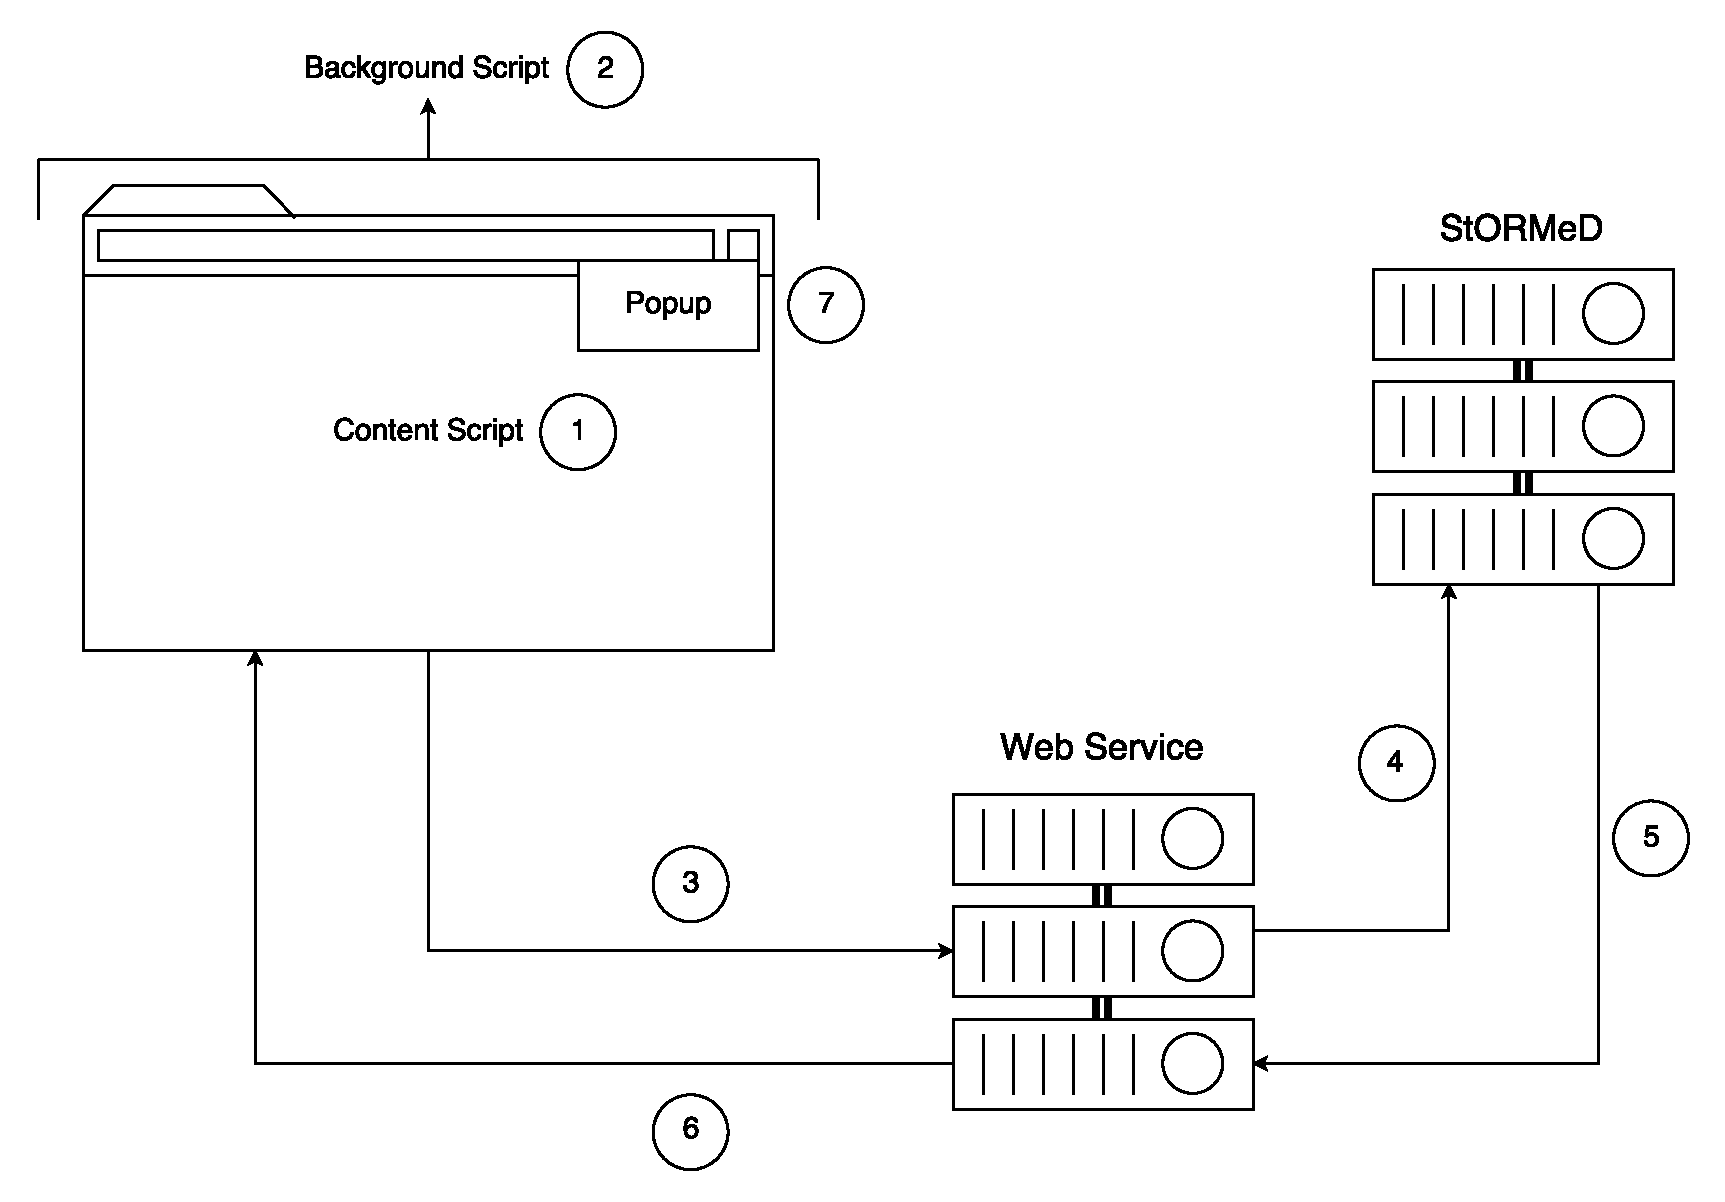
\includegraphics[scale=0.4]{Figures/Architecture}
\caption{Architecture of \projectName}
\label{fig:architecture}
\end{figure}
Each of these numbers will be explained in a later section. In the next few sections, we will analyse each component, and its specific tasks.

\subsubsection{Parser}
The first step consists in collecting the information currently being displayed, which happens when the page has finished loading its content. As previously discussed\todo{Add reference}, one of the main challenges of this project was to handle the wide variety of structures among webpages, being as each page tends to use the same constructs but widely differ in the implementation. This hurdle was solved by implementing a parser for each of the domains for which the information was needed. 

\begin{figure}[H]
\centering
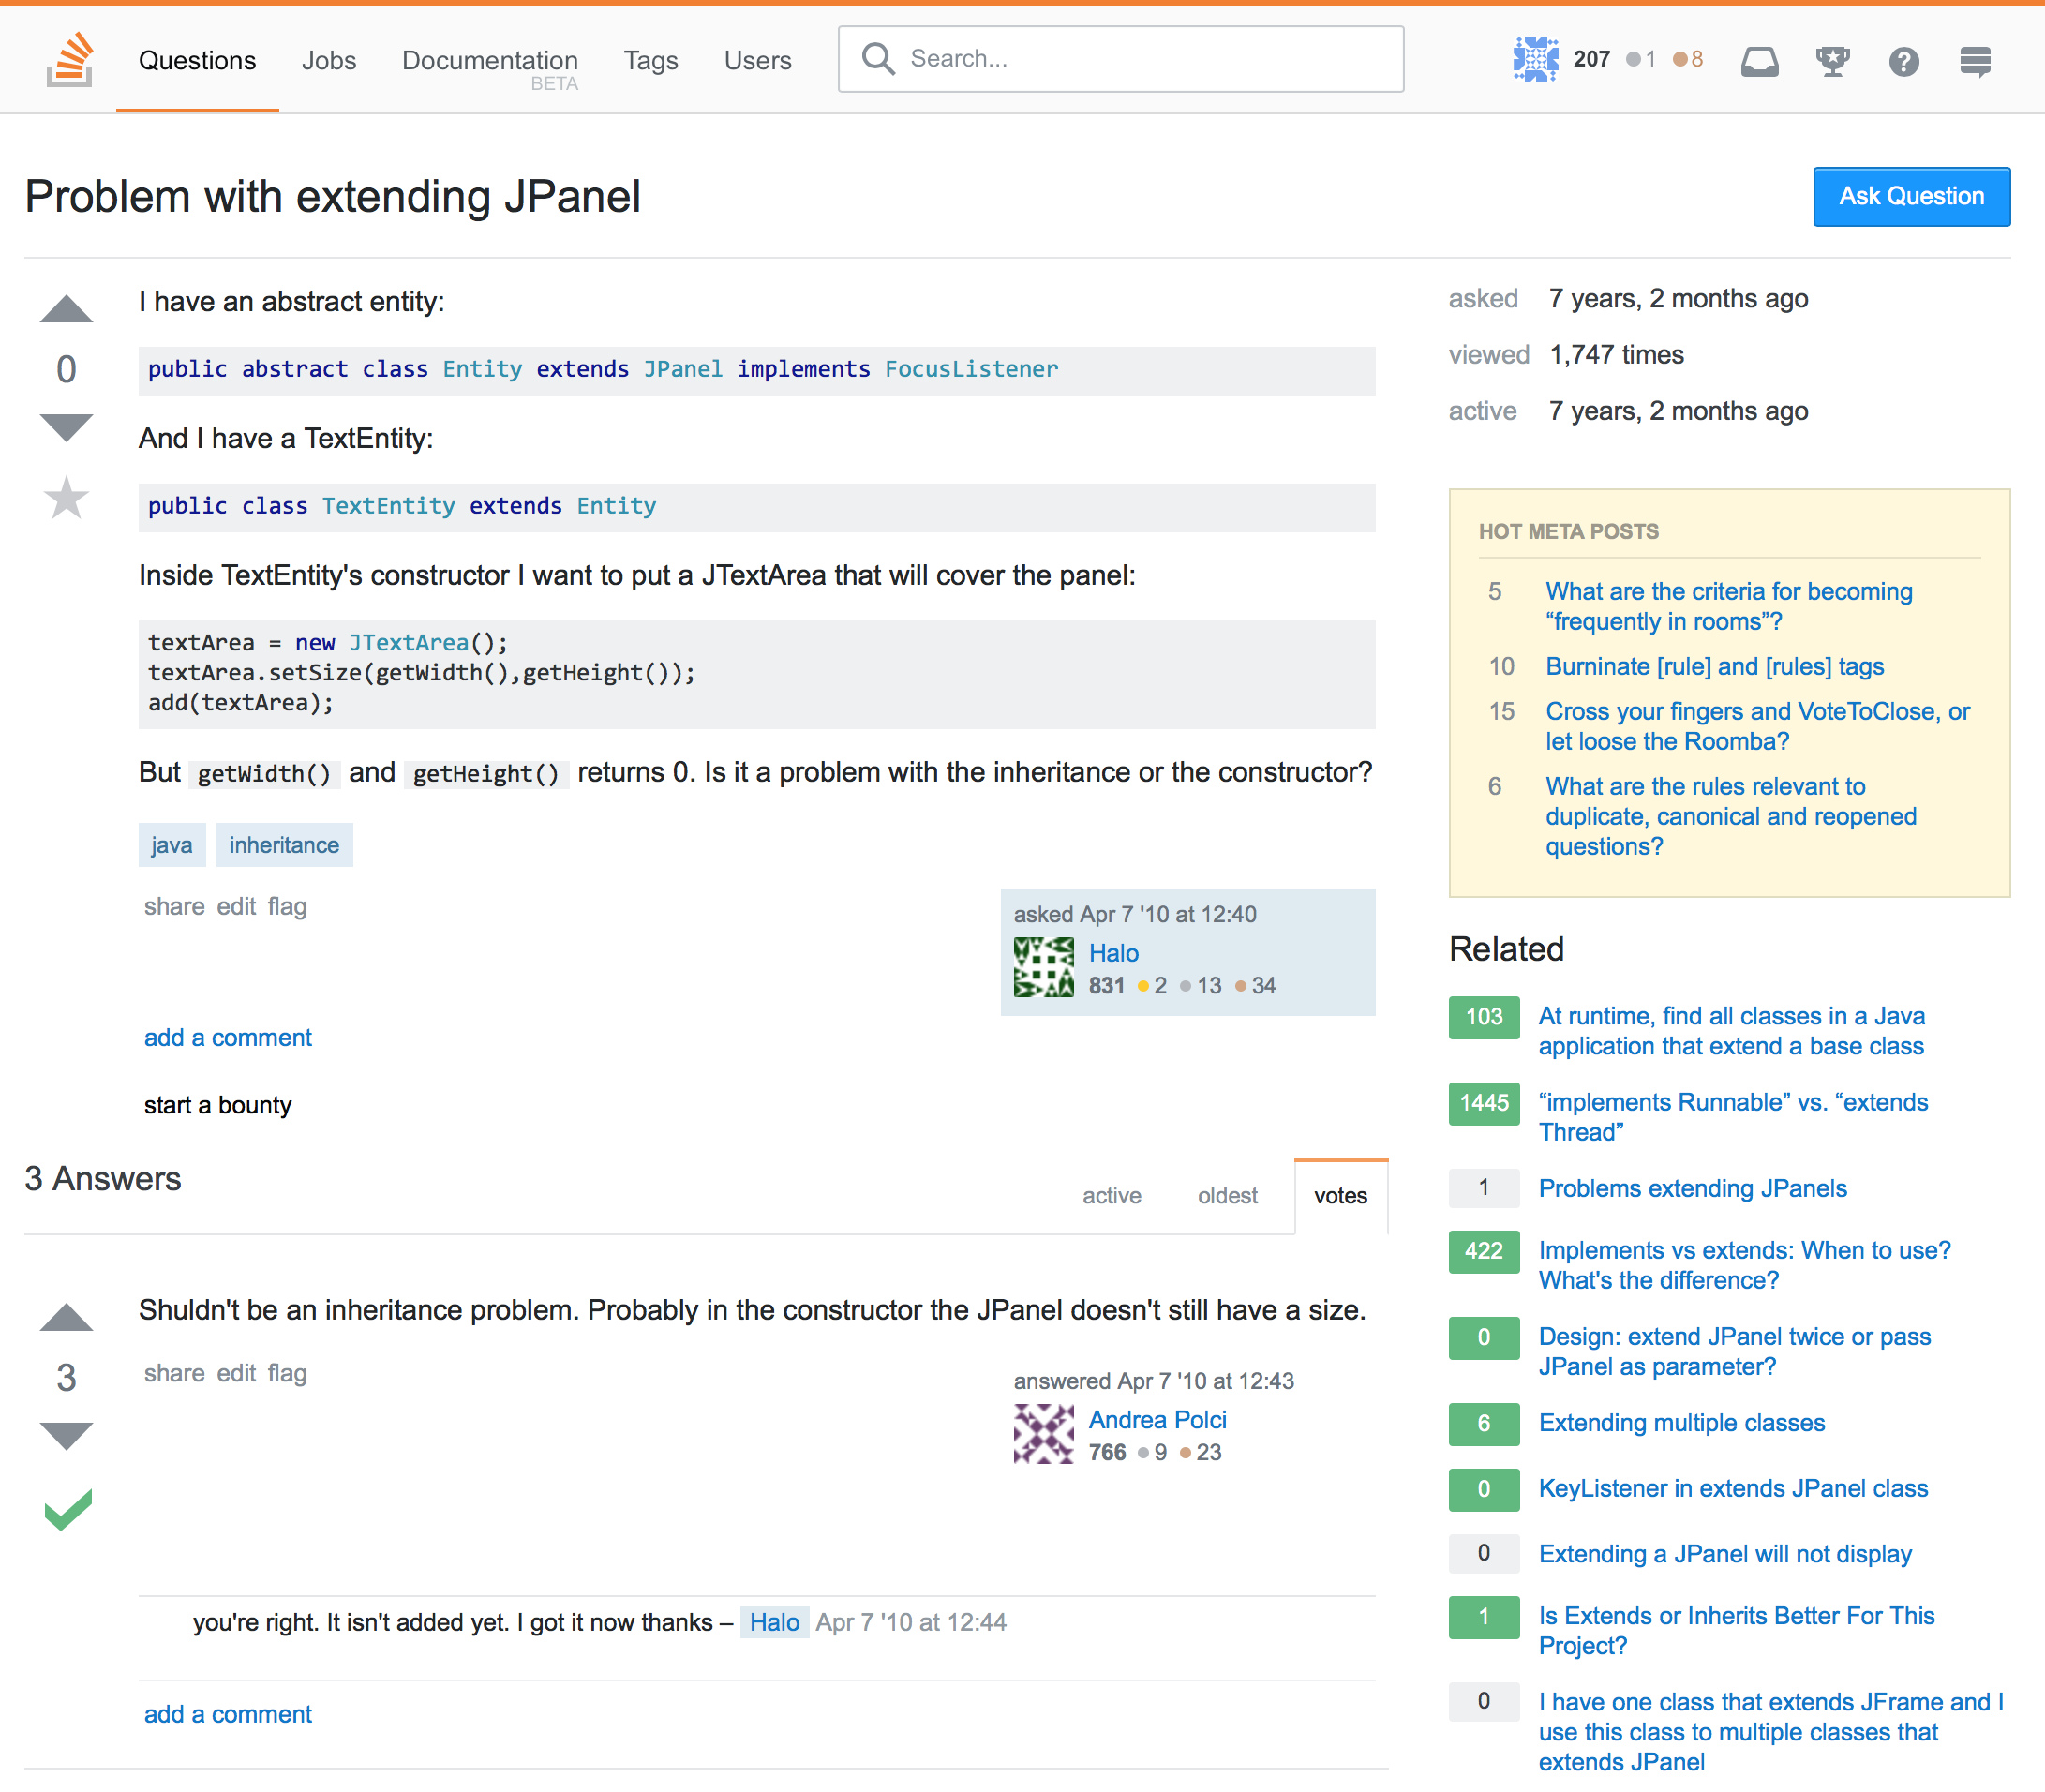
\includegraphics[scale=0.3]{Figures/SOConv}
\caption{A typical StackOverflow conversation}
\label{fig:soConv}
\end{figure}

Figure \ref{fig:soConv} represents the structure of a StackOverflow conversation. It is easy to see that there is a set structure which consists of a question, and $0$ or $n$ answers. Therefore our parser needs to first obtain the question, more specifically the paragraphs that make up such question, and then repeat the task for each of the possible answers. 

In order to classify these pieces of information, we introduce the notion of an information unit. An information unit is a piece of content extracted from a page, which contains either text or code. The distinction has to be made when the content is extracted, in order to keep the integrity of code in such a way that it may be used later on by a simple copy and paste approach. 

To ease the process of writing a parser, an abstract parser was created, with a few models to accompany the methods. Being as the parser has to live inside of the browser extension, the language sed to write such a program is JavaScript. Although a pretty complete programming language \todo{CRINGE}, the current version as of writting this document is ES5\todo{Sure?}, which does not yet support features such as classes, inheritance, and more. Being as our implementation is supposed to be abstract, meaning that for each domain this parser can be extended, we needed a language that could support inheritance. After a bit of research, the choice ended up being TypeScript\footnote{\url{https://www.typescriptlang.org}}, a language developed by Microsoft which is a typed superset of JavaScript that compiles to plain JavaScript. This ensured that compatibility would not be an issue, while providing multiple useful features. 

\begin{figure}[H]
\centering
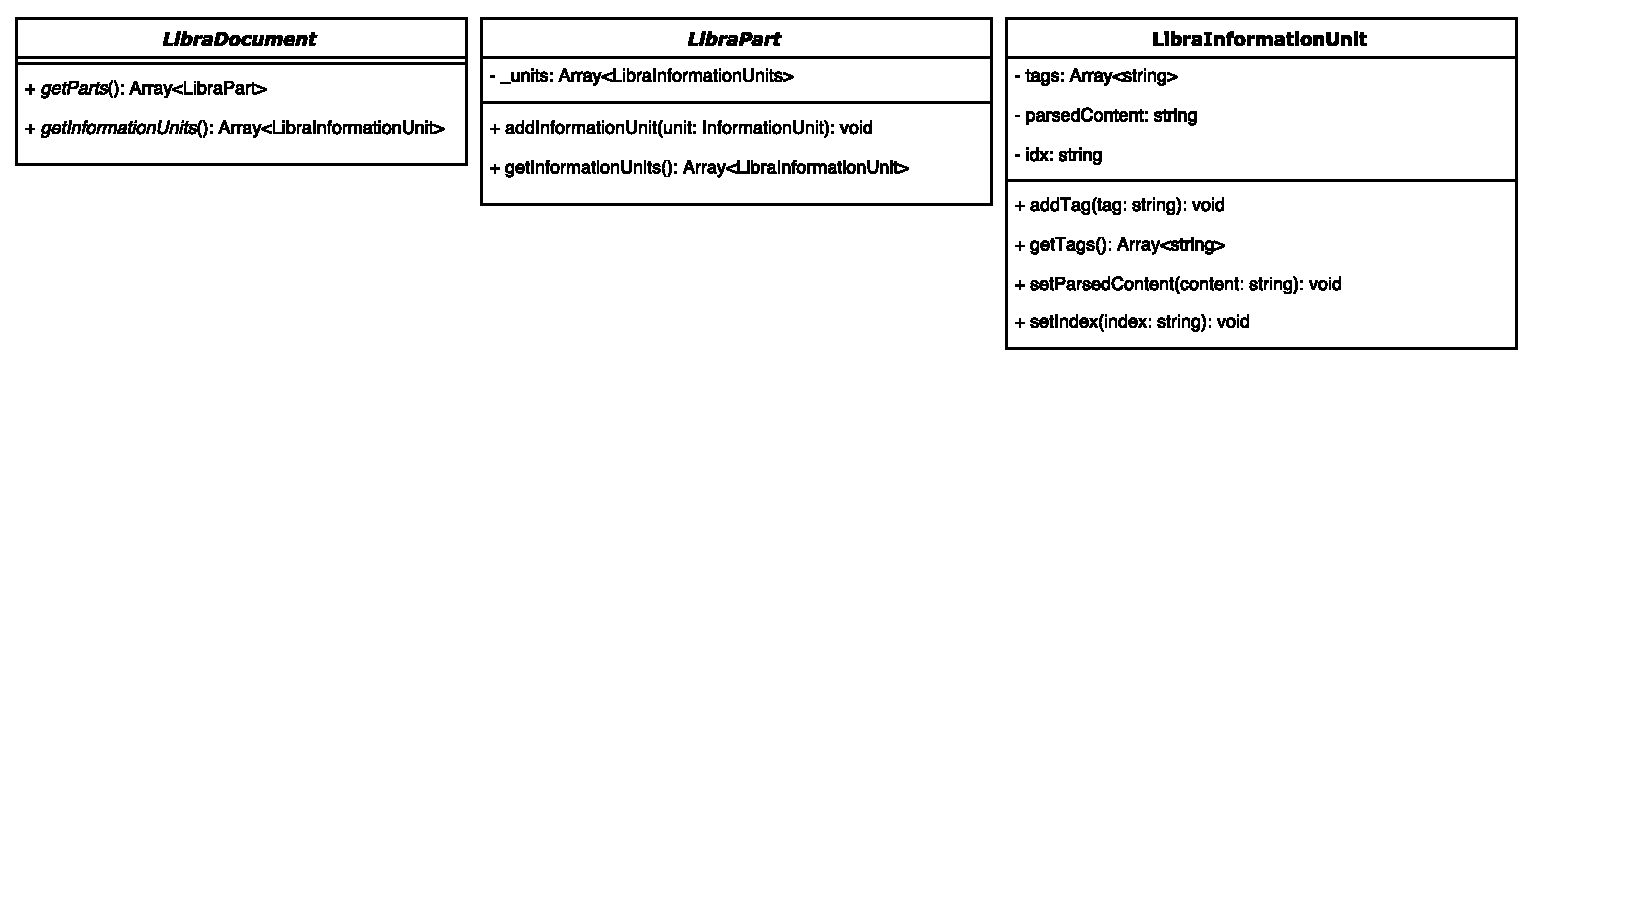
\includegraphics[scale=0.5]{Figures/ClassUML}
\caption{Abstract parser class diagram}
\label{fig:abstractParserClassDiagram}
\end{figure}


We started by defining the models that would be needed to parse a page. A document diagram can be found in Figure \ref{fig:abstractParserClassDiagram}.

The ``root'' model is called \ts{LibraDocument} which provides the main methods that will be called by the extension, namely \ts{parse()} and \ts{getInformationUnits()}. Then, the information unit is defined, which encapsulates the data required to run the analysis. The last piece is \ts{LibraPart}, which allows us to separate the multiple parts of a document. As an example, consider the previously shown StackOverflow conversation. We could divide the question and the answers in two separate parts, which themselves contain other parts (i.e. the possible answers). 

\begin{figure}[H]
\centering
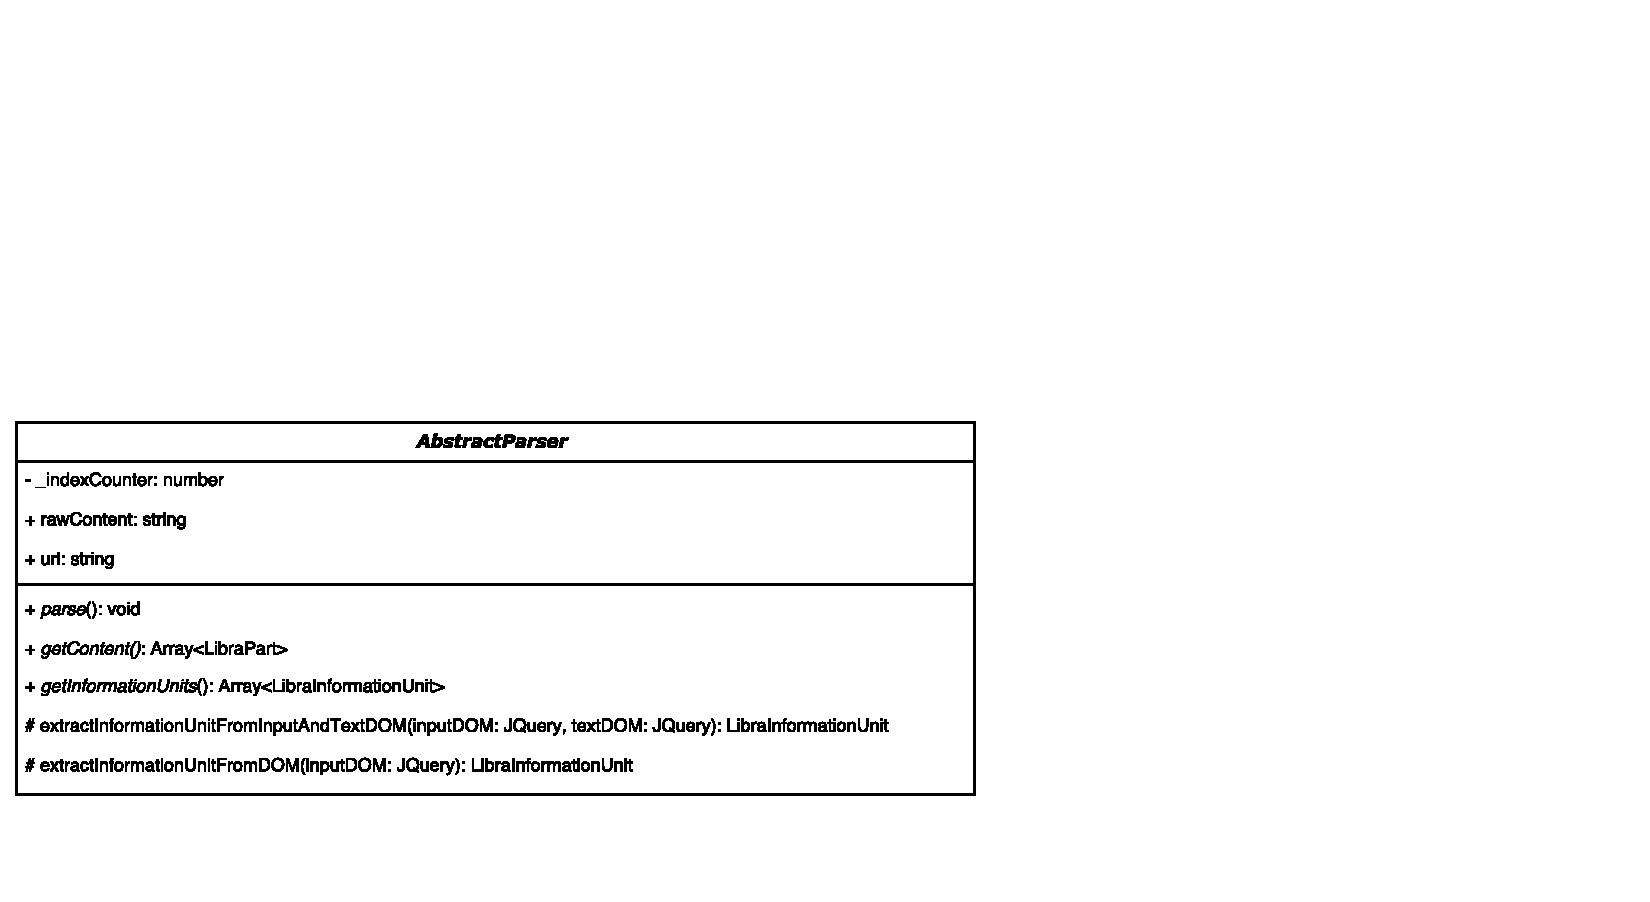
\includegraphics[scale=0.5]{Figures/AbstractParserUML}
\caption{Abstract parser}
\label{fig:abstractParserDiagram}
\end{figure}

These models are then used in the abstract parser, for which the diagram is show in figure \ref{fig:abstractParserDiagram}. This way the developer writing a new parser has to simply extend the different methods and models, quickly creating a new parser which the extension is able to understand and use. 

A remark ha to be made about the \ts{extractInformationUnitFromDOM} and \ts{extractInformationUnitFromInputAndTextDOM} methods. These two methods were created to keep the way that the data is extracted consistent among multiple parser implementations. The two methods are almost identical, and work in the following way:

\begin{enumerate}
	\item A small marker, comprised of the URL hash combined with the current counter inside the document is injected into the HTML tags containing the information, like so:
\begin{htmlcode}
<pre class="lang-java prettyprint prettyprinted" libra_idx="-656298628_0000000001">
    ...
</pre>
\end{htmlcode}
\item The counter is then increased
\item The type of the content, text or code, is identified and attached inside of the information unit
\item The information unit is returned to the developer
\end{enumerate}
The reason why we are injecting the index is quite simple. In order to identify the unit to which a certain degree belongs to, we need to leave small traces such as this index, being as the service does not return the parsed text, but only the index and degree. This procedure is explained more in details in section \todo{Needs ref}. The index construction needed to abide to certain constraints, namely the ability of being unique inside a document, as well as when doing multiple document summarisation. In the end, the approach we chose was as follows:
\[
\text{\texttt{Hash of url + "\_" + 10 digit padded index}}
\]
Although hashing may introduce cases where the produced hash is not unique, the probability of such an event occurring was small enough to be ignored.


By creating the two methods in \ts{LibraDocument} as abstract, each parser can implement their own, while allowing the extension to call the same methods, regardless of the page being viewed (and hence parser being used), while effectively providing a common interface to the parser. 

The execution of the parser is performed once the loading of the page is completed, which itself fires the request to the web service, discussed in this next section.

\subsubsection{Web Service}
The second main component of this project consists in a web service, that takes the information units given by the extension, and returns the degree of centrality for each of the information units. This service was written in Scala, using the Play framework. Most of the code is written in a functional way\todo[inline]{Can this be said?}, which proved to be quite the challenge but very satisfying when things were working correctly. 

The service has the following routes:

\begin{itemize}
\item \texttt{GET /register}\\
Used to register the user to the service. This is needed as to identify the user in all subsequent calls to the service. The response is a 32-character string, which contains both numbers and letters. Once the user registers, a graph is created unique to this id, allowing for subsequent information units to be added, and therefore the ranking to be performed depending on the entire graph, not only the current units being analysed.
\item \texttt{POST /rank}\\
This path is used to rank the current units extracted from a document. By supplying the url of the webpage, the units, and the user id header, the service will return the units with a degree of centrality. 
\texttt{GET /all}\\
Returns the entire graph for a certain user, with all units associated with their degree of centrality.
\end{itemize}

\noindent In figure \ref{fig:architecture} the entire architecture is shown. An example workflow\todo{This does not sound good} is as follows:
\begin{enumerate}
\item User install the extension, opens it for the first time which prompts the registration procedure
\item The user id is stored in storage, for later use
\item The user navigates to a known page, which fires the content script's parsing process (Label 1)
\item Once parsing is completed, the background script takes over and prepares the data to be sent (Label 2)
\item The data is sent to the web service, which starts processing (Label 3) \label{item:serviceRequest}
\item The service sends a part of the data over to the island parser (Label 4)
\item Once the data is returned (Label 5), if it is the first request for that particular user, the graph is created
\item The nodes are added to the graph, and ranking starts \label{item:serviceRank} 
\item Once completed, the data is returned to the background script, which notifies the popup that the data is ready (label 6) \label{item:serviceReturn}
\item The popup prepares itself, and the user ca now interact with it (Label 7)
\end{enumerate}

In this section we are going to focus on points \ref{item:serviceRequest}, \ref{item:serviceRank}, and \ref{item:serviceReturn}. When the extension makes the request, a few pieces of informations are needed. The following is an example of the request:
\begin{jsoncode}
POST /rank
Content-Type: application/json
X-Libra-UserId: SsrktS2vrGPpHaAkYMsVDPo4qN6i38ei

{
  "units": [
    {
      "idx": "-656298628_0000000001",
      "parsedContent": "Creating an instance of a class:",
      "tags": [
        "plaintext"
      ]
    },
    {
      "idx": "-656298628_0000000002",
      "parsedContent": "MyObject myObject = new MyObject();",
      "tags": [
        "code"
      ]
    }
  ],
  "url": "http://www.MyAwesomeWebsite.rocks"
}
\end{jsoncode}

As we can see, the request requires the content type, the user id when registration happens, as well as the units with the url. 


Once the units are received, the service will fire a request for each of the units to the StORMeD\cite{Ponz2015b} service. This service is an island parser, which will allow us to construct the full AST from a certain unit. 

The service will then add the nodes to the graph, and start calculating the degree by using a library called Signal/Collect\cite{Stutz:2010:SGA:1940281.1940330}, which allows the processing of large graphs in a really quick way. By describing the HoliRank algorithm using the provided syntax, the library handles the calculations returning the degree of centrality for a certain unit. The results are then returned to the user in the following format:
\begin{jsoncode}
{
  "units": [
    {
      "idx": "-656298628_0000000001",
      "degree": 0.5,
      "url": "http://www.MyAwesomeWebsite.rocks"
    },
    {
      "idx": "-656298628_0000000002",
      "degree": 0.5,
      "url": "http://www.MyAwesomeWebsite.rocks"
    }
  ]
}
\end{jsoncode}

This information is then used by the extension to associate the index with its degree, which is then used to decide which units have to be hidden and which have to be shown depending on the value chosen by the user. This is explained in details in the next section.

\subsection{Chrome Extension}
As previously stated, in order to parse the content of a certain page, send it to the service, and then manipulate it, a Chrome extension was created. The extension encapsulates three main components:
\begin{itemize}
\item \textbf{Content Script}\\
The content script has the task of loading the available parser, as well as using such parser. Once this is completed, the data is handed over to the background script.
\item \textbf{Popup}\\
The popup is the only piece of this project which a user can see. It is the main point of interaction between the user and the project. She has the ability to choose the amount of information that has to be displayed. 
\item \textbf{Background script}\\
The background script has the task of connecting the content script with the popup. 
\end{itemize}
Before we go any further, one must understand how a Chrome extension works. As with our implementation, an extension usually consists of three main components as described above. These components have different restrictions regarding what data they can access, how they are instantiated, and when they are destroyed. 

The background script is persistent, meaning it stays alive for the duration of the session, and has the ability to make HTTP requests but has no access to the content on the page, or the content of the popup. On the other hand, the content script has the ability to access the content, but no access to the popup. Last but not least, the popup is recreated every time the user clicks on the icon, and has no access to the content. This means that the three components have to communicate to each other, by means of message passing. 

Each of these components has the ability to send and receive messages, and react accordingly. This was useful when, for example, the user had just registered to the service. Each component has its own localStorage, but the user id had to be used by multiple components which created an issue regarding where to store it. In the end message passing was used and a common local storage was chosen, this being the background script's storage as this component was always listening and active.


As we have seen in the previous section, the service returns the payload containing the different degrees of each unit. It is the task of the extension as a whole to process this information, and make it usable to the user. This is achieved by sorting the payload data, and adding in each of the units currently on the page a sort order index, as follows:
\begin{htmlcode}
<pre class="lang-java prettyprint prettyprinted" libra_idx="-656298628_0000000001" sortorder="15">
	...
</pre>	
\end{htmlcode}
Once this manipulation is complete, the popup updates its view, and shows a range slider, allowing the end user to choose the percentage of the information that she may want to be displayed. Every time the value of the slider changes, the popup fires a message, calling into action the content script which will hide or show the units depending on their sort order. The interface is shown in figure \ref{fig:chromeExtensionInterfaceScreenshot}

\begin{figure}[H]
\centering
\missingfigure{Screenshot of the extension with the popup open and bar dragged}	
\caption{Interface of the Chrome extension}
\label{fig:chromeExtensionInterfaceScreenshot}
\end{figure}

Another feature of the extension, is the ability of generating a page containing all the units that have been visited by a certain user. If the user clicks on the summary button, a new page is opened containing all of the units, and for each site a range slider is added to choose the amount of information displayed. An additional range slider is added at the top of the page, called a master slider, which controls the amount of information displayed by each site, regardless of the value chosen by each individual slider. This allows the user to consult only the highest ranked units in a website, giving a very quick overview of multiple sites at the same time. The result can be seen in figure \ref{fig:chromeExtensionSummaryScreenshot}

\begin{figure}[H]
\centering
\missingfigure{Screenshot of the Summary	}
\caption{Generated Summary}
\label{fig:chromeExtensionSummaryScreenshot}
\end{figure}

\section{Implementation Issues}\label{sec:implementationIssues}

\subsection{Current Limitations}
\subsubsection{Granularity}
Although this approach to summarisation works, the biggest limitation is the granularity of it. As we have seen, the service is able to correctly identify the importance of each unit inside of a document or collection of documents, but what is still missing is a true summarisation of the content. More specifically, what would be interesting to achieve is a summarisation algorithm that is able to take a text, and recreate a new one by following grammar rules and keeping the context of such intact.

Although interesting, it would bring a new set of challenges, particularly when dealing with code that is embedded inside of a sentence, forcing it to be shown no matter what in the summary. Making the summariser understand exactly how to connect code and text may prove to be quite the challenge

\subsubsection{Persistence}
The current implementation of the web service uses an in memory store, meaning that there is no real database behind the service, and the data is kept in memory and destroyed once the service is shut down. Although not essential to the project, a database would be useful, allowing the user to retrieve data that is older than what is saved in current memory. 

This brings the challenge of deciding what has to be kept, what has to be discarded and when. By keeping all of the units stored in a database, the user may see information that is too old or has nothing to do with the current context. A new way to tag the information would be required, tagging what the context was, when the information unit was added, and whether to discard it once new units are added to the current graph.

\subsubsection{Performance}
To implement the algorithm behind \projectName, many libraries were used. These libraries tend to have their own way of doing things, which our code had to adapt to. One example is the \scala{SimilarityParameters} present in the StORMeD devkit. These parameters have to be recalculated every time a new unit is added, which requires a lot of time. If we were only to consider small graphs, this would be no problem as there is almost no impact on the general performance. Once we start to consider larger graphs, the limitations start to show, and the performance of the whole system suffers. In order to fix such issue, the devkit would have to be rewritten from scratch, which is outside the scope of this project. 

\subsection{Future work}
\section{Results}\label{sec:results}
The goal of this project was to provide a simple way for developers to reduce information overload. It was very important that the user interface of the Chrome extension was as simple as possible to remove any possible hurdles. Figure \ref{fig:chromeExtensionInterfaceScreenshot} shows the user interface for the popup component of the Chrome extension. 

\begin{figure}[H]
\centering
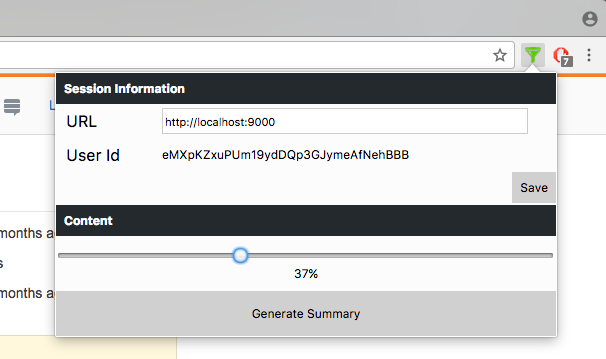
\includegraphics{Figures/ChromeUI}
\caption{Interface of the Chrome extension}
\label{fig:chromeExtensionInterfaceScreenshot}
\end{figure}

The interface consists of two main sections. The first section shows information about the current session. This was mostly used while debugging the application. The second section is used to interact with the user. The current view shows the slider, which means that the data gathering and ranking processes have completed successfully. In case of errors, or while the content script is parsing the page, the slider is hidden and messages are shown to inform the user of the current status. 

An additional visual feedback is provided by the possible icons of the extension shown in Figure \ref{fig:icons}, which can represent any of the following states:
\begin{itemize}
\item \textbf{Inactive}\\
Represented by a greyed out icon (Figure \ref{fig:chromeInactive}), tells the user that the extension is not active in the current website.
\item \textbf{Parsing}\\
While the application is parsing, a yellow icon (Figure \ref{fig:chromeParsing}) is shown to indicate that the Chrome extension is working, and the results will be shown shortly.
\item \textbf{Ready}\\
When the icon turns green (Figure \ref{fig:chromeReady}), the user has the ability to open the popup and start manipulating the content by dragging the slider.
\item \textbf{Error}\\
If an error occurs, a red icon is shown (Figure \ref{fig:chromeError}). 
\end{itemize}
\newcommand{\figureScale}{0.25}
\newcommand{\innerScale}{0.15}


\begin{figure}[H]
\centering
\begin{subfigure}[b]{\figureScale\textwidth}
\centering
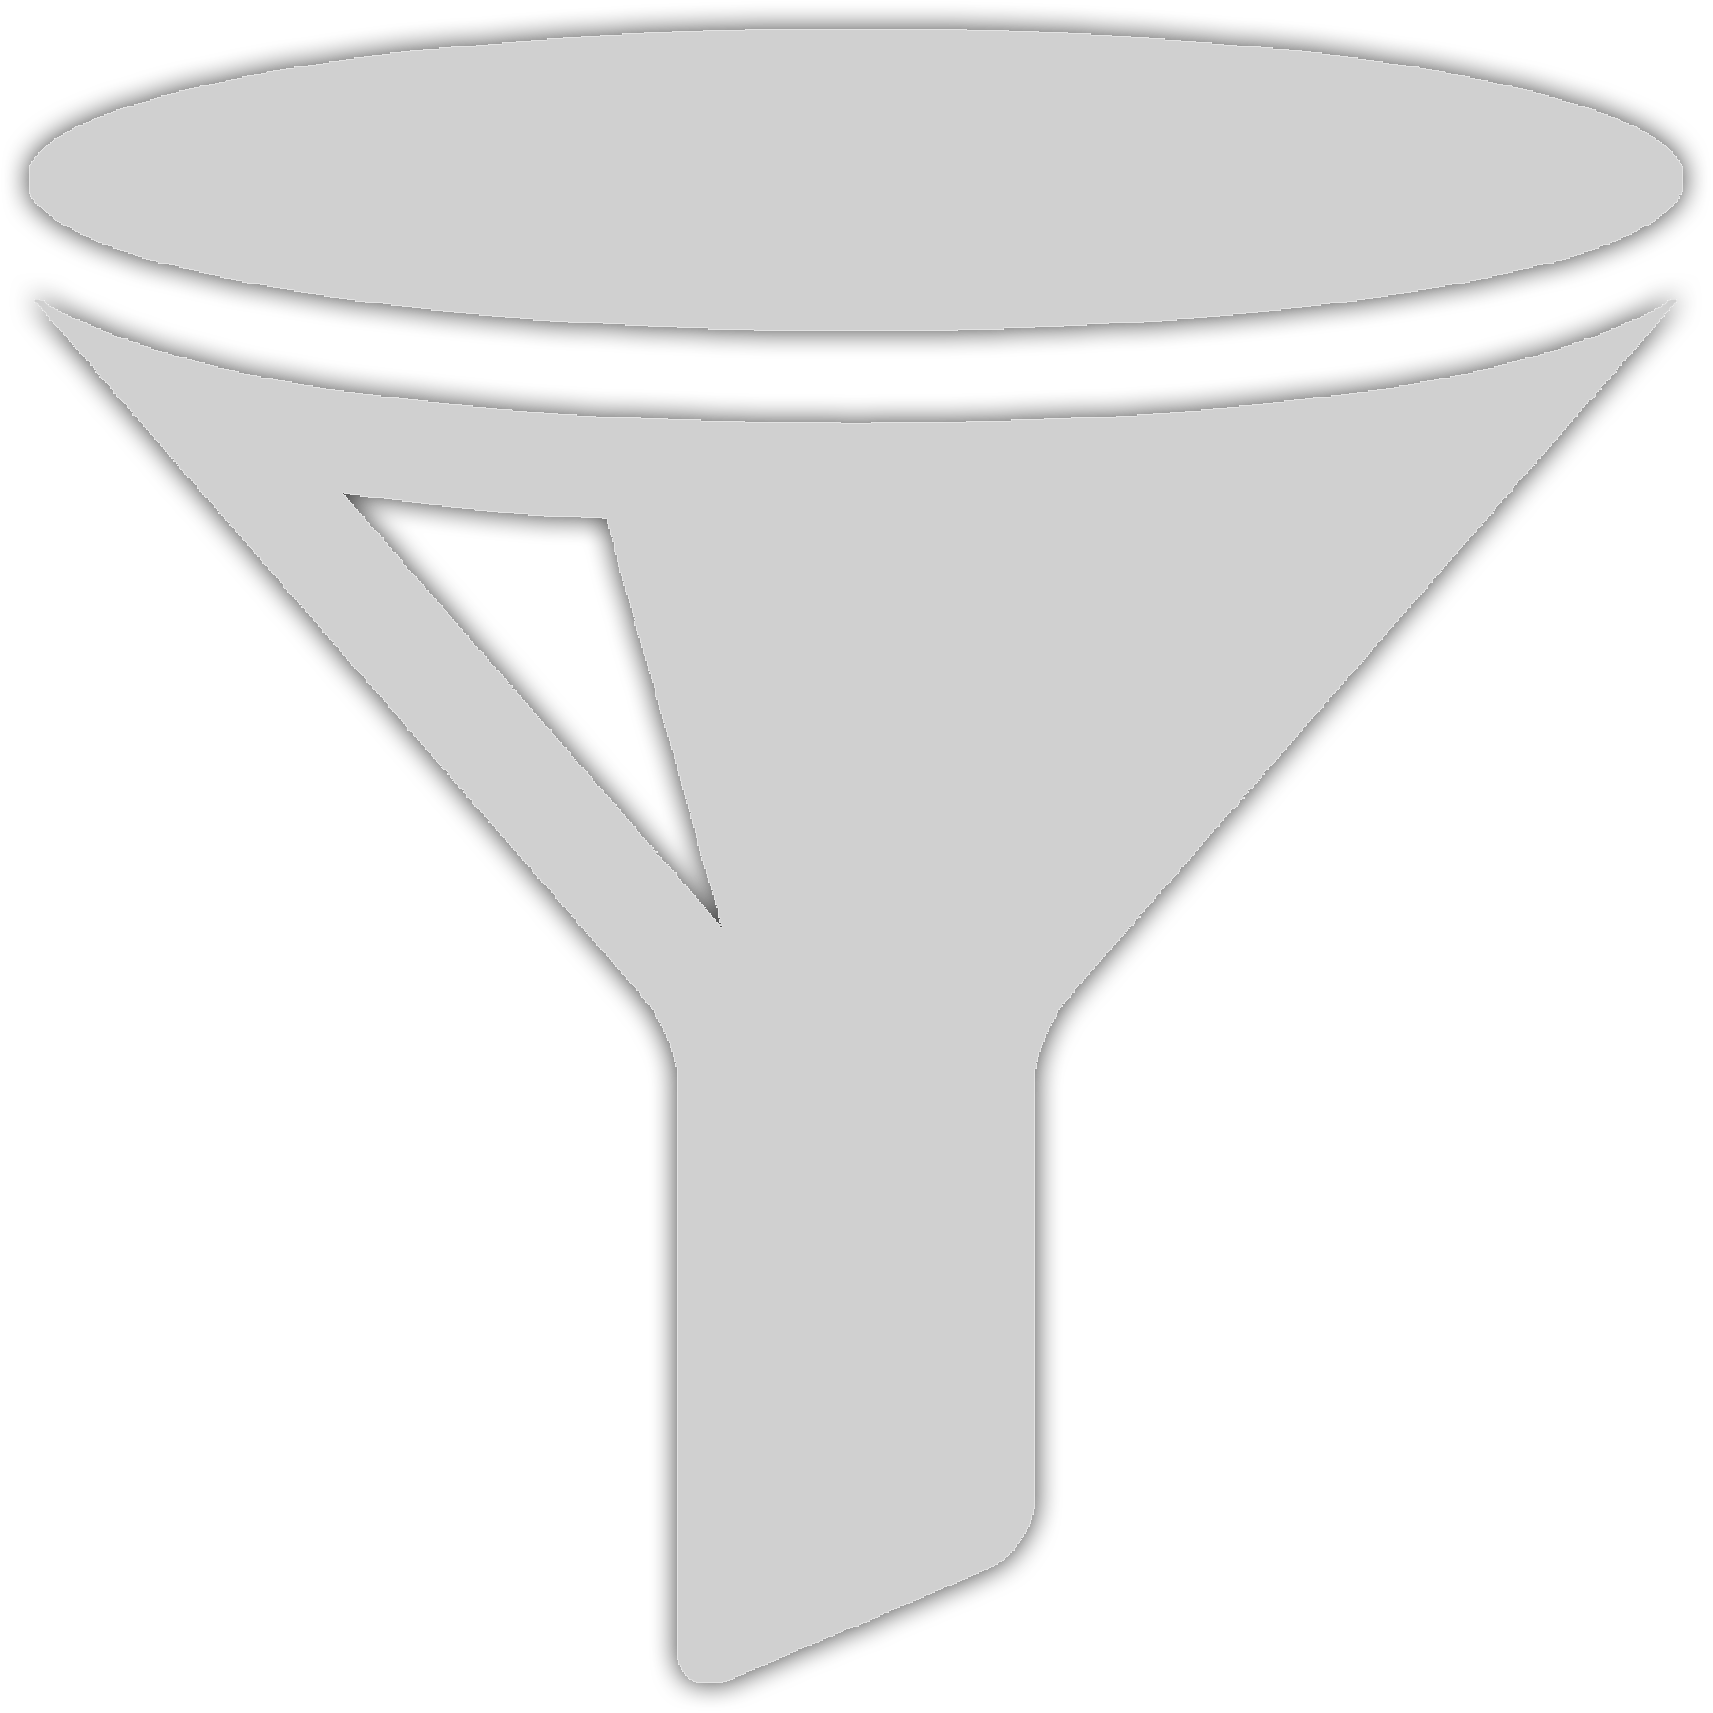
\includegraphics[scale=\innerScale]{Figures/greyPlain}
\caption{Inactive}
\label{fig:chromeInactive}
\end{subfigure}~
\begin{subfigure}[b]{\figureScale\textwidth}
\centering

\includegraphics[scale=\innerScale]{Figures/yellowPlain}
\caption{Parsing}
\label{fig:chromeParsing}
\end{subfigure}~
\begin{subfigure}[b]{\figureScale\textwidth}
\centering

\includegraphics[scale=\innerScale]{Figures/greenPlain}
\caption{Ready}
\label{fig:chromeReady}
\end{subfigure}~
\begin{subfigure}[b]{\figureScale\textwidth}
\centering

\includegraphics[scale=\innerScale]{Figures/redPlain}
\caption{Error}
\label{fig:chromeError}
\end{subfigure}
\caption{Chrome extension status icons}\label{fig:icons}
\end{figure}

When the Chrome extension has received the data back from the web service, the icon turns green and the slider is shown in the popup. The user has now the ability to choose the amount of filtration required, which updates the content of the page in real time. Any time the slider is dragged, the popup will fire an event caught by the content script, which will take care of hiding or showing the different units, depending on their sort order.


Another feature of \projectName~is the ability to generate an overview of all the pages in a user's history. By clicking the Generate summary button from the popup (Figure \ref{fig:chromeExtensionInterfaceScreenshot}), the extension will open a new page, containing the documents. An example is shown in Figure \ref{fig:chromeExtensionSummaryScreenshot}.
\begin{figure}[H]
\centering
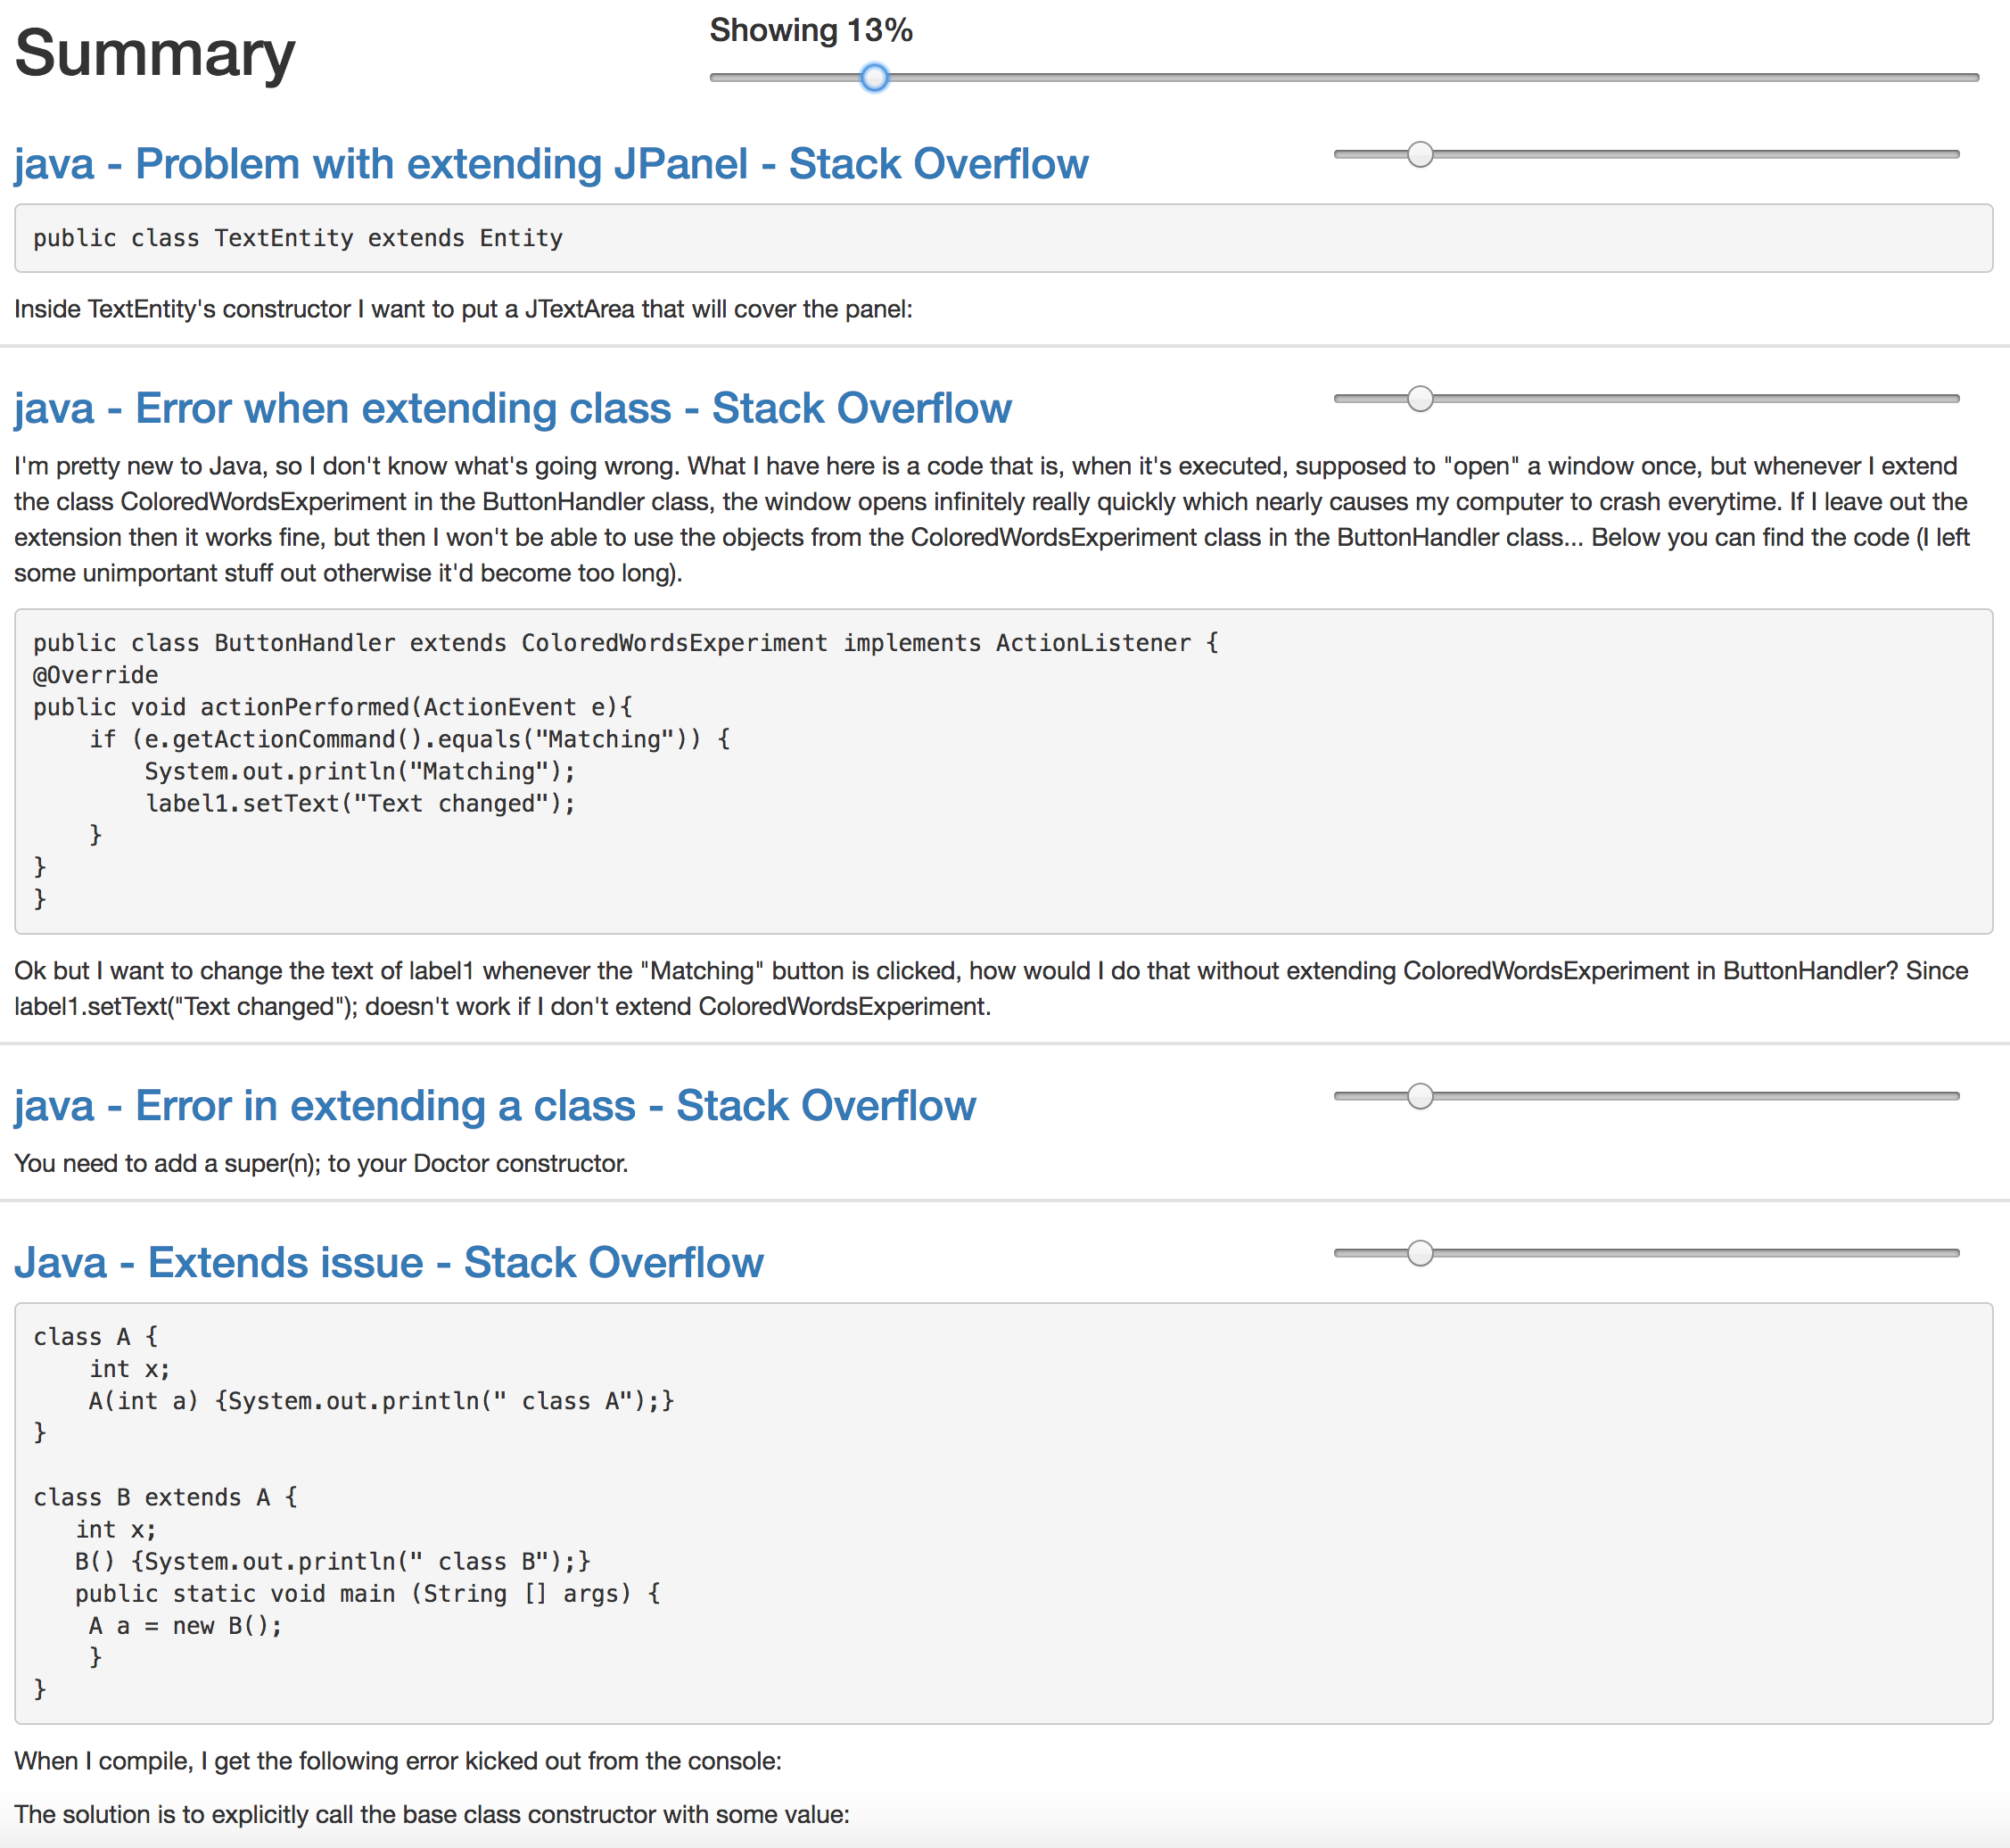
\includegraphics[scale=0.3]{Figures/SummaryExample}
\caption{Generated Summary}
\label{fig:chromeExtensionSummaryScreenshot}
\end{figure}

For each page, a slider is available to once again filter the content independently from the other pages. An additional slider is added at the top of the page, called a master slider, which controls the amount of information displayed by each site, regardless of the value chosen by each individual slider. This allows the user to consult only the highest ranked units in its history, giving a very quick overview of multiple sites at the same time.

\section{Conclusion}\label{sec:conclusion}
We presented WebDistiller, a novel approach to reducing information overload. It is the combination of a holistic ranking approach, with a simple to use UI. Developers have now the ability to partially offload the task of filtering the content, allowing them to focus on the task at hand. By also providing a summary functionality, we provide the ability to see the previously seen pages, with an easy to use interface that allows them to filter the content once again, with the importance of each section based on the entire history, and not only the current document. 










\newpage
%%%%% BIBLIOGRAPHY %%%%%
\bibliographystyle{abbrv}
\bibliography{Other/references}

\end{document}